\documentclass[a4paper]{article}

\usepackage[margin=1.5cm]{geometry}
\usepackage{amsmath,amsthm,amssymb,tabu}
\usepackage[spanish,es-tabla]{babel}
\decimalpoint
\usepackage[T1]{fontenc}
\usepackage[utf8]{inputenc}
\usepackage{lmodern}
\usepackage[dvipsnames]{xcolor}
\usepackage[hyphens]{url}
\usepackage{graphicx}
\graphicspath{ {images/} }
\usepackage{tcolorbox}
\usepackage{enumitem}
\setcounter{section}{-1}
\usepackage{tabularx}
\usepackage{multirow}
\usepackage{hyperref}
\usepackage{braket}
\usepackage{tikz}
\usepackage{mathrsfs}
\usetikzlibrary{cd}
\usepackage{pgfplots}
\usepackage{caption}
\usepackage{subcaption}
\usetikzlibrary{babel}

\definecolor{NARANJA}{rgb}{1,0.467,0}
\definecolor{VERDE}{rgb}{0.31,1,0}
\definecolor{AZUL}{rgb}{0,0.53,1}
\definecolor{ROJO}{rgb}{1,0,0}


\hypersetup{
    colorlinks=true,
    linkcolor=ROJO,
    filecolor=magenta,
    urlcolor=AZUL,
}
\newenvironment{theorem}[2][Theorem]{\begin{trivlist}
\item[\hskip \labelsep {\bfseries #1}\hskip \labelsep {\bfseries #2.}]}{\end{trivlist}}
\newenvironment{teorema}[2][Teorema]{\begin{trivlist}
\item[\hskip \labelsep {\bfseries #1}\hskip \labelsep {\bfseries #2.}]}{\end{trivlist}}
\newenvironment{lema}[2][Lema]{\begin{trivlist}
\item[\hskip \labelsep {\bfseries #1}\hskip \labelsep {\bfseries #2.}]}{\end{trivlist}}
\newenvironment{exercise}[2][Exercise]{\begin{trivlist}

\item[\hskip \labelsep {\bfseries #1}\hskip \labelsep {\bfseries #2.}]}{\end{trivlist}}
\newenvironment{problem}[2][Problem]{\begin{trivlist}
\item[\hskip \labelsep {\bfseries #1}\hskip \labelsep {\bfseries #2.}]}{\end{trivlist}}
\newenvironment{question}[2][Question]{\begin{trivlist}
\item[\hskip \labelsep {\bfseries #1}\hskip \labelsep {\bfseries #2.}]}{\end{trivlist}}
\newenvironment{corollary}[2][Corollary]{\begin{trivlist}
\item[\hskip \labelsep {\bfseries #1}\hskip \labelsep {\bfseries #2.}]}{\end{trivlist}}
\newenvironment{corolario}[2][Corolario]{\begin{trivlist}
\item[\hskip \labelsep {\bfseries #1}]}{\end{trivlist}}
\newenvironment{solution}{\begin{proof}[Solution]}{\end{proof}}

\pgfplotsset{compat=1.15}

\begin{document}
\title{Proyecto Intermedio. Algoritmos Computacionales}
\author{Diego Alberto Barceló Nieves  \\ Mauricio Sandoval Cuenca \\ Facultad de Ciencias \\ Universidad Nacional Autónoma de México}
\date{}
\maketitle

Elige 2 de los 3 problemas que se muestran a continuación y entrega las soluciones en un notebook con código de julia a más tardar el 5 de mayo de 2022. 


\section*{Ejercicio 1} \label{Sec: Ejercicio 1}

El triángulo de Sierpinski es un fractal convergente a un conjunto fijo con la figura de un triángulo equilátero subdividido recursivamente en triángulos equiláteros más pequeños. Éste es uno de los ejemplos más básicos de conjuntos \textit{autosemejantes} (se dice que un objeto es autosemejante cuando una o varias partes de un todo repiten exactamente su similitud con ese todo) ver Figura \ref{fig:sierp_0}. Existen distintos algoritmos que nos permiten obtener el triángulo de Sierpinski, a continuación describimos uno de los más sorprendentes:

\begin{enumerate}
    \item Sin dibujarlos, considera tres puntos en un plano que formen los vértices de un triángulo equilátero.
    \item Elige un punto arbitrario dentro de la superficie del triángulo equilátero y considéralo tu \textit{posición actual}.
    \item Elige de forma aleatoria uno de los tres vértices del triángulo equilátero.
    \item Obtén el punto medio entre tu posición actual y el vértice que elegiste en el paso anterior, considéralo tu nueva posición actual.
    \item Dibuja el punto de tu posición actual.
    \item Repite desde el paso 3.
\end{enumerate}

El ejercicio consiste en implementar el algoritmo anterior y obtener una aproximación del triángulo de Sierpinski. Más aún, juega con el número de vértices iniciales y la distancia de la posición actual al vértice elegido para obtener un fractal distinto. Como seguramente podrás notar, no todas las combinaciones devuelven un fractal.

\begin{figure}[h!]
    \centering
    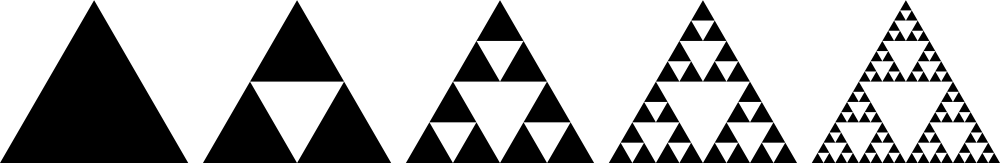
\includegraphics[width=.8\linewidth]{img/sierp.png}
    \caption{Triángulo de Sierpinski}
    \label{fig:sierp_0}
\end{figure}

\textbf{Hint.} En Julia puedes utilizar la función \texttt{rand()} para generar un número entero aleatorio dentro de un rango.


\section*{Ejercicio 2} \label{Sec: Ejercicio 2}

En el rodaje de una película de acción, se busca encontrar cuál es el piso más alto de un edificio de 100 niveles desde el que puede saltar el stuntman sin provocar un accidente. Para esto, el equipo cuenta con dos maniquíes para ensayos de colisiones que pueden dejar caer desde cualquier piso y se saben las siguientes cosas:

\begin{enumerate}
    \item Si el maniquí se rompe al caer del piso $n$, entonces es no seguro que el stuntman salte desde ese nivel ni en ninguno posterior.
    \item Si el maniquí no se rompe al caer del piso $n$, entonces es seguro que el stuntman salte desde ese nivel y en cualquiera inferior.
    \item Si el maniquí no se rompe después de ser lanzado, entonces puede ser usando de nuevo para otra prueba.
    \item Un maniquí roto no puede volver a usarse.
    \item No se tiene seguro que el maniquí no se dañe al caer desde el primer piso, ni es totalmente seguro que se dañará al caer del último piso.
\end{enumerate}

El equipo no puede permitir que el stutman salté de un piso sin tener total certeza de que es seguro. La forma más inmediata de encontrar el máximo piso seguro desde el que puede saltar es probando de uno en uno, sin embargo, en el peor de los casos les tomaría 100 intentos.

Una forma más ágil de resolver el problema es aprovechando el hecho de que tienen dos maniquíes de prueba haciendo una \textit{búsqueda binaria}. Se empieza desde el piso 50, si el maniquí no se rompe se vuelve a probar pero ahora desde el piso 75, sin embargo si el maniquí se rompe, entones se tendrá que probar uno por uno desde el primer piso y en el peor de los casos tomaría 49 intentos.

Se puede probar que para dos maniquíes y 100 pisos, la mejor solución se obtiene empezando desde el piso 14, teniendo que en el peor de los casos tomaría máximo 14 intentos encontrar el piso indicado. Para este ejercicio, escribe un algoritmo que devuelva el mínimo número de intentos necesarios (en el peor de los casos) teniendo $n$ maniquíes y un edificio de $k$ pisos.


\section*{Ejercicio 3} \label{Sec: Ejercicio 3}

Un método para estimar el valor de $\pi$ ($3.141592...$) es usando el método de Monte Carlo. Tomando un cuadrado de 1 $\times$ 1 y un círculo inscrito de radio $\frac{1}{2}$, generamos una cantidad arbitraria de puntos uniformemente distribuidos sobre la superficie del cuadrado y coloremos de rojo aquellos que se encuentren sobre la superficie del círculo y de azul aquellos que estén fuera como se muestra en la Figura \ref{fig:pi}.

\begin{figure}[h!]
    \centering
    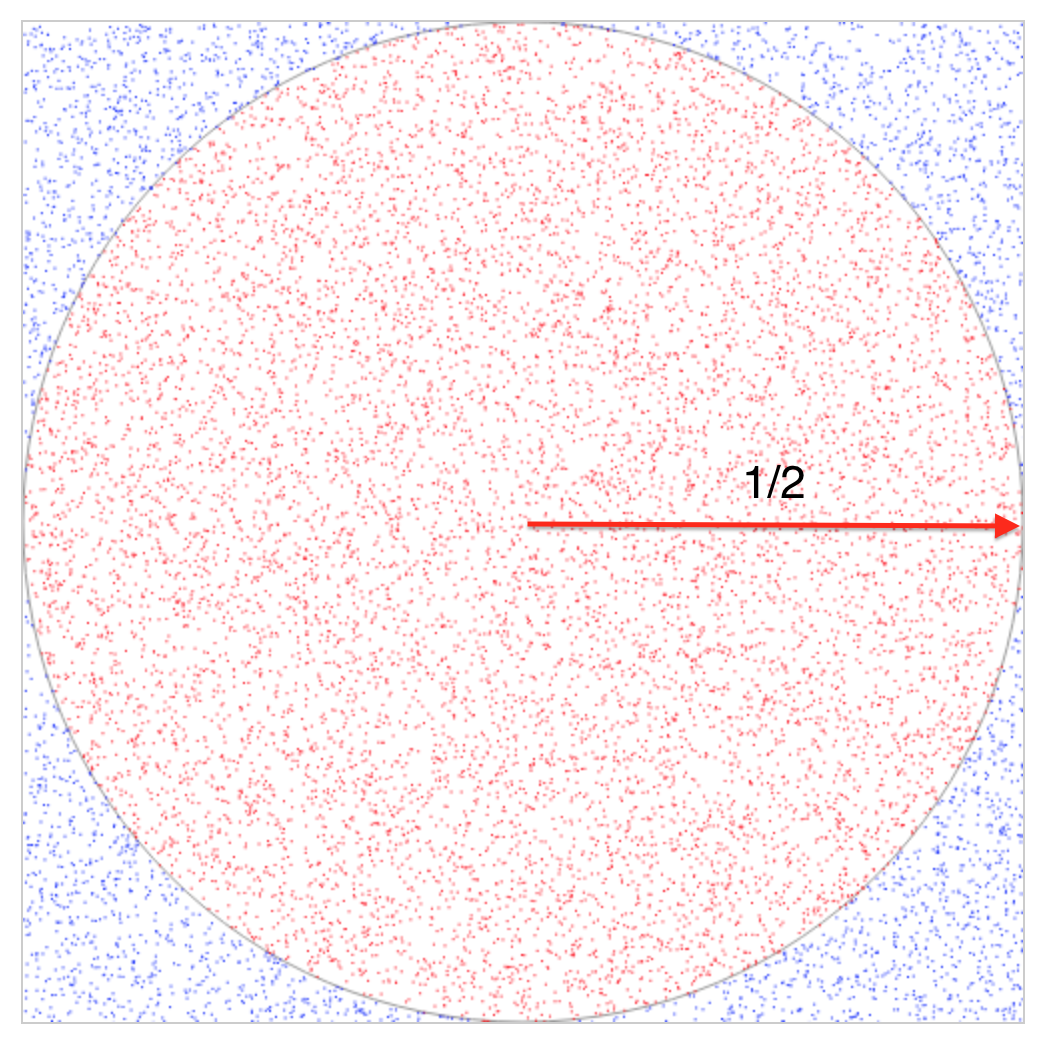
\includegraphics[width=.4\linewidth]{img/pi.png}
    \caption{Aproximación de pi por el método de Monte Carlo}
    \label{fig:pi}
\end{figure}

Tenemos que el área del círculo esta dada por $\pi r^2 = \frac{\pi}{4}$, mientras que el área del cuadrado es igual a $1$. Si dividimos el área del círculo entre el área del cuadrado obtenemos $\frac{\pi}{4}$, además si $N_{rojo}$ es el número de puntos rojos y $N_{total}$ es el número total de puntos, entonces $\frac{N_{rojo}}{N_{total}}$ debería ser una aproximación del cociente de las áreas para $N_{total}$ lo suficientemente grande, en otras palabras

\begin{align*}
    & \frac{\pi}{4} \approx \frac{N_{rojo}}{N_{total}} \\
    \Rightarrow & \ \pi \approx 4\ \frac{N_{rojo}}{N_{total}}
\end{align*}

La última ecuación nos da la estimación de $\pi$ por el método Monte Carlo.

\begin{enumerate}
    \item Escribe un algoritmo que estime el valor de $\pi$ y que te permita visualizar algo similar al gráfico de la Figura \ref{fig:pi}, asegúrate de incluir el conteo del número de puntos rojos, número de puntos totales y la respectiva estimación de $\pi$.
    \item En promedio, ¿cuántos puntos necesitas generar para obtener una precisión del 0.01? \textbf{Observación:} Al tratarse de un método aleatorio, los resultados variarán de una ejecución a otra, por eso es importante tomar el promedio u otro estadístico.
    \item Realiza una gráfica del error de la estimación en función del número de puntos comparando contra el valor predeterminado de pi de julia (lo puedes obtener llamando a la constante predeterminada \texttt{pi}).
\end{enumerate}


\end{document}
